\chapter{Data Penelitian}

\section{Data Simulasi IES-VE}
Data penelitian ini dapat diakses di \textit{http://bit.ly/DataSkripsiS1Ridhan}

\begin{table}[!h]
	\caption{Data Simulasi IES-VE}
	\label{tbl:A:DataSkripsiRidhan}
	\centering
	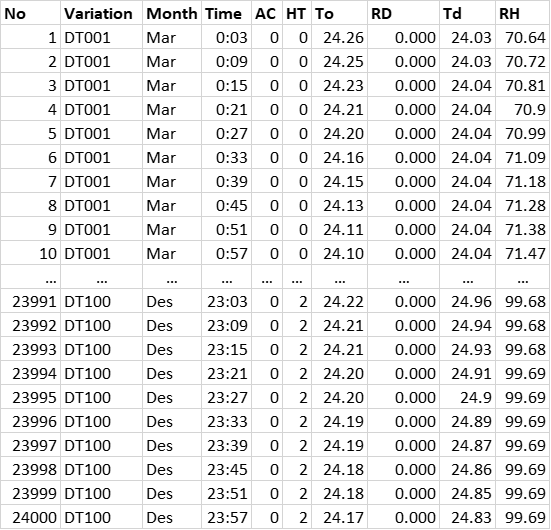
\includegraphics[width=0.75\textwidth]{figures/DataSkripsiRidhan}
\end{table}
\vspace{3em}
\break
\break

\section{Bobot-bobot Model JST Kontroler}
\begin{table}[!h]
	\caption{Bobot-bobot Model JST Kontroler}
	\label{tbl:A:BobotKontroler}
	\centering
	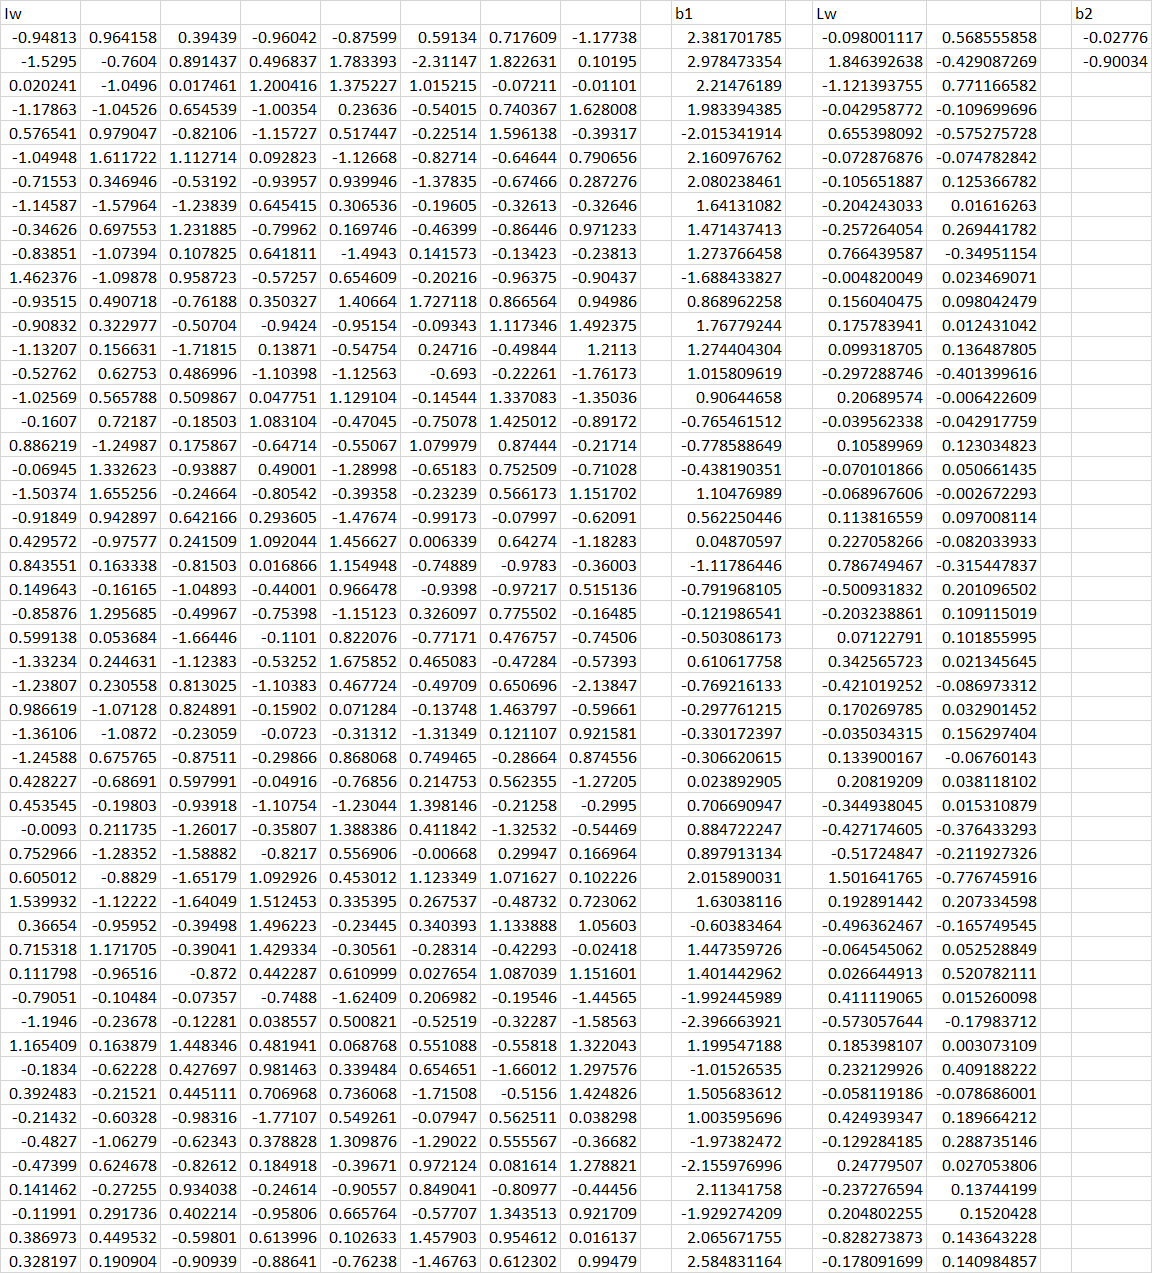
\includegraphics[width=1\textwidth]{figures/BobotKontroler}
\end{table}
\vspace{1em}
\break

\section{Hasil Simulasi Sistem Kontrol}
\begin{table}[!h]
	\caption{Hasil Simulasi Sistem Kontrol}
	\label{tbl:A:HasilSimulasiKontrol1}
	\centering
	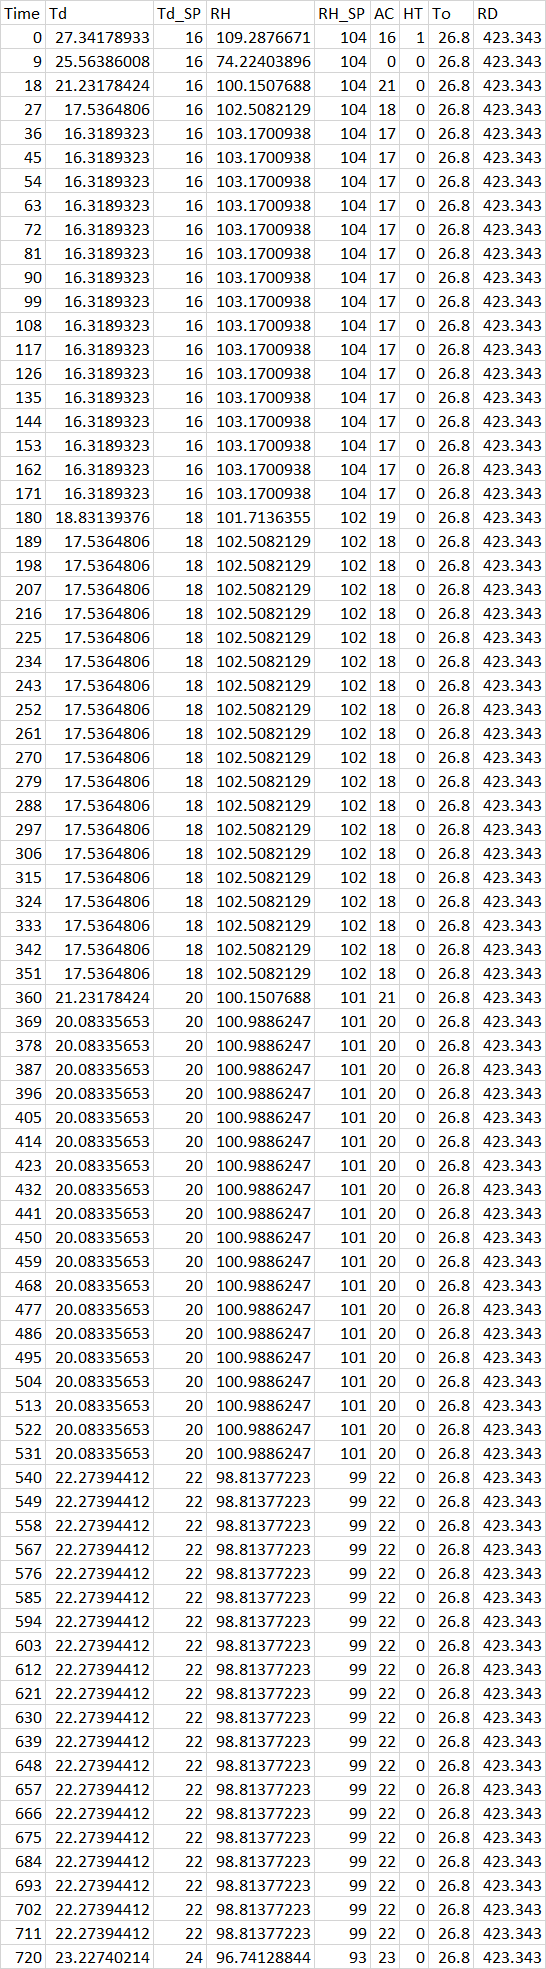
\includegraphics[width=0.34\textwidth]{figures/HasilSimulasiSimulink1}
\end{table}
\break

\section{Hasil Simulasi Sistem Kontrol (lanjutan 2)}
\begin{table}[!h]
	\caption{Hasil Simulasi Sistem Kontrol}
	\label{tbl:A:HasilSimulasiKontrol2}
	\centering
	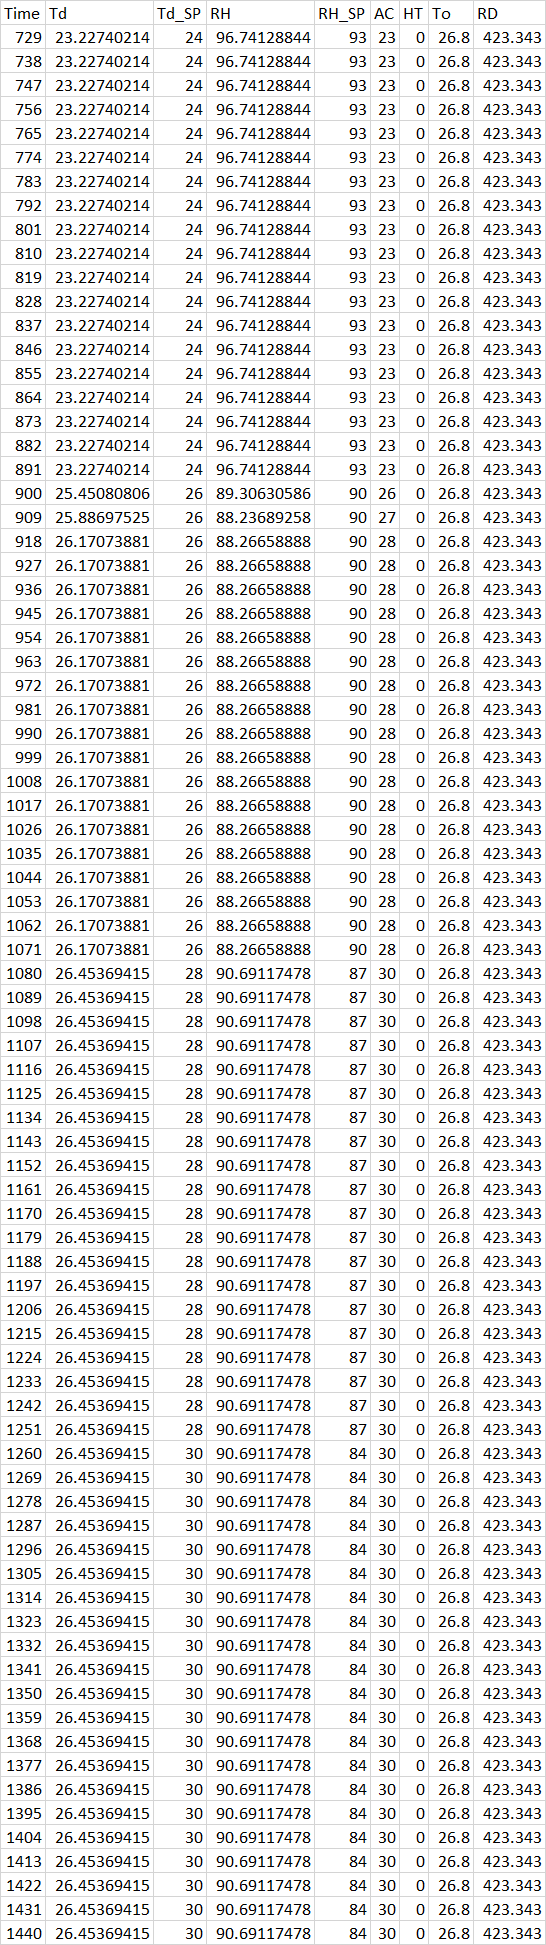
\includegraphics[width=0.35\textwidth]{figures/HasilSimulasiSimulink2}
\end{table}
\break

\section{Hasil Simulasi Sistem Kontrol (lanjutan 3)}
\begin{table}[!h]
	\caption{Hasil Simulasi Sistem Kontrol}
	\label{tbl:A:HasilSimulasiKontrol3}
	\centering
	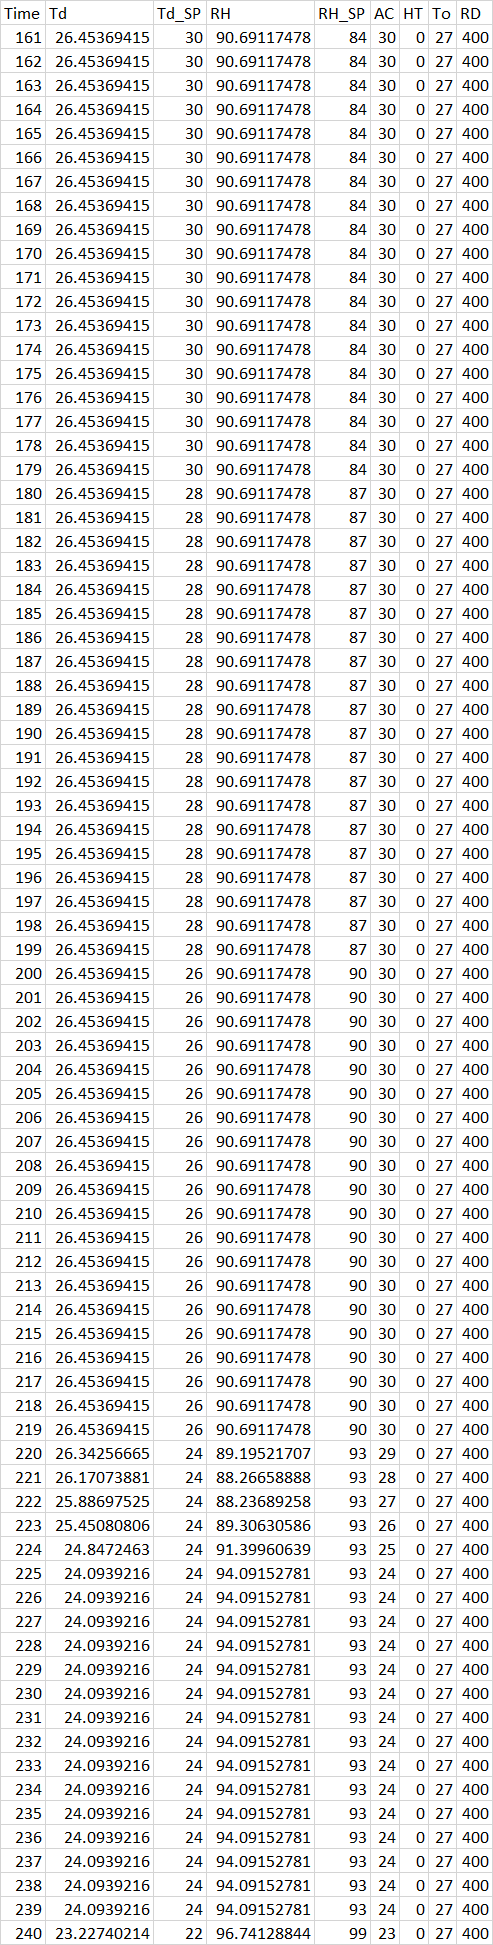
\includegraphics[width=0.35\textwidth]{figures/HasilSimulasiSimulink3}
\end{table}
\break

\section{Hasil Simulasi Sistem Kontrol (lanjutan 4)}
\begin{table}[!h]
	\caption{Hasil Simulasi Sistem Kontrol}
	\label{tbl:A:HasilSimulasiKontrol4}
	\centering
	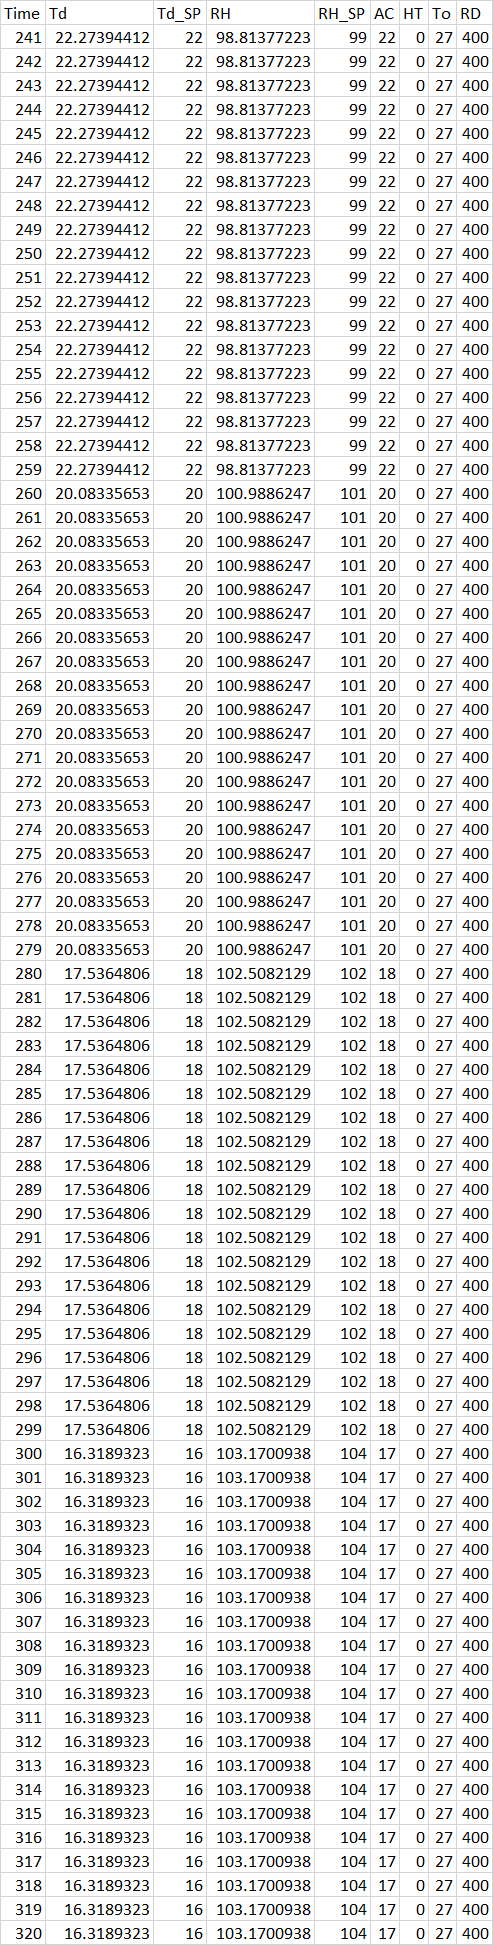
\includegraphics[width=0.35\textwidth]{figures/HasilSimulasiSimulink4}
\end{table}